\apendice{Especificación de diseño}

\section{Introducción}

Tras el estudio de los requisitos se pasa a un diseño, en este apéndice se explicarán los distintos diseños de la aplicación, desde los datos, los procesos más importantes, el diseño arquitectónico y las interfaces.

\section{Diseño de datos}

De los requisitos y casos de usos se deduce el diseño de los datos. Para poder cumplir correctamente con las necesidades del cliente se introducen dos entidades, los \textbf{usuario} y las \textbf{camas} en la que cada uno almacena la información relevante propia. A su vez se relacionan en el sistema de permisos de que persona puede ver que cama. El diagrama Entidad-Relación se puede observar en la figura~\ref{fig:erDia}

\begin{figure}
	\centering
	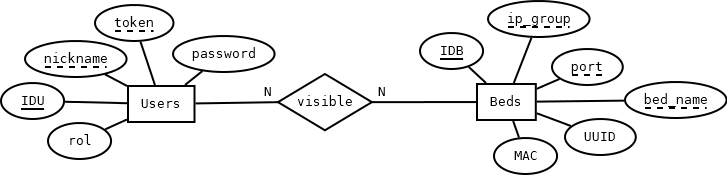
\includegraphics[width=\textwidth]{img/entidad-relacion.png}
	\caption{Diagrama entidad-relación}
	\label{fig:erDia}
\end{figure}

De este diagrama generamos el diagrama relacional (figura~\ref{fig:relational}) en el que se especifican las tablas que se usarán en el producto final.

\begin{figure}
	\centering
	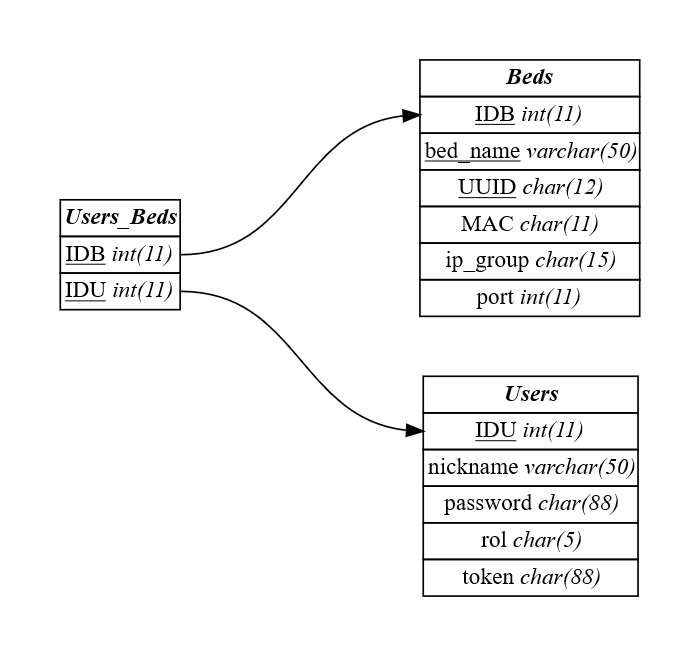
\includegraphics[width=0.5\textwidth]{relational}
	\caption{Diagrama relacional}
	\label{fig:relational}
\end{figure}


\section{Diseño procedimental}\label{sec:disproc}

Existen diversos procesos importantes en la aplicación. El primero es la creación de los componentes que se encargan de monitorizar las camas, como se puede observar en la figura~\ref{fig:proc_sec}. Al principio, el servidor instancia todos los \textit{BedListener} necesarios según las camas que existan, y estos instancian su \textit{BedProcess} correspondiente. Es importante destacar que estas dos clases funcionan como hilos. 

\begin{figure}
	\centering
	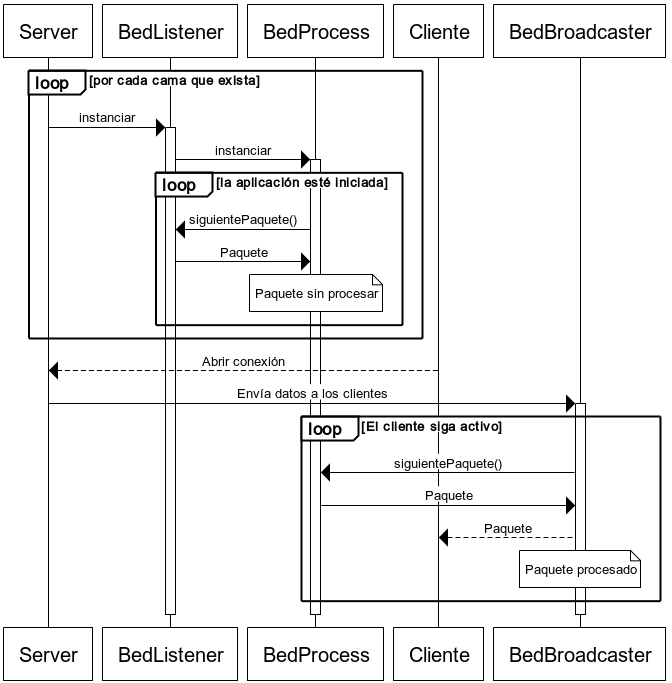
\includegraphics[width=\textwidth]{proc}
	\caption{Diagrama de secuencias de la creación de camas y la petición de paquetes}
	\label{fig:proc_sec}
\end{figure}

Por otra parte el cliente abre conexiones con el servidor solicitando datos, este genera un hilo del \textit{BedBroadcaster} que existe mientras el cliente esté activo (el que comenzó la petición o cualquiera que se incorpore posteriormente). 

El proceso completo de la conexión del cliente se puede ver en la figura~\ref{fig:ws-secuence}. En esta cada llamada es un \textbf{evento} de \textit{socketio} y los argumentos los datos que espera. 

\begin{figure}
	\centering
	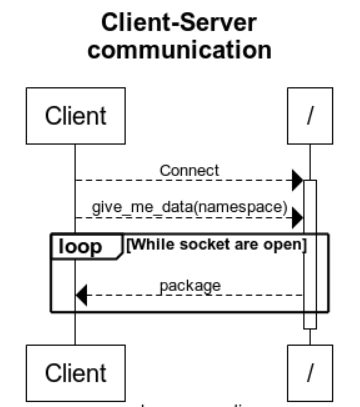
\includegraphics[width=0.5\textwidth]{img/ws-secuence.png}
	\caption{Comunicación cliente servidor \textit{websocket}}
	\label{fig:ws-secuence}
\end{figure}

Los procedimiento de toda la \textit{API} se especifican luego en la sección~\ref{sec:api}.

\section{Diseño arquitectónico}

La arquitectura software sigue el patrón \textit{MVC}~\cite{wiki:mvc}. Sin embargo, al ser un problema sencillo no se traslada a un diseño literal de este patrón. El \textit{modelo} se mantiene en la base de datos y no tiene una representación en ninguna clase. El \textit{controlador} está pensado en varios componentes, una \textit{API} que gestiona todo los accesos a la base de datos y un \textit{proxy} que recoge las peticiones web y las preprocesa para redirigirlas a la \textit{API}. Por último, la \textit{vista} puede ser completamente diseñada para la situación que se requiera, en esta aplicación se gestiona mediante plantillas \textit{HTML} y peticiones \textit{AJAX} ya que se trata de una aplicación web. Gracias a que el controlador funciona como una \textit{API REST} esta vista puede ser cambiada según se desee.

Otra arquitectura relevante es el \textit{pipeline} de procesamiento de los datos de pacientes. Se puede observar, junto con los módulo de \textit{routing}, en la figura~\ref{fig:classes}. Se trata de tres componentes, dos con contexto en toda la aplicación, que se trata del \textit{listener} de la cama y el procesador de la misma. El último es el \textit{broadcaster} que emite los datos a los pacientes. En la sección~\ref{sec:disproc} se puede ver la comunicación del cliente y el proceso de inicialización de los componentes de este \textit{pipeline}.

\begin{figure}
	\centering
	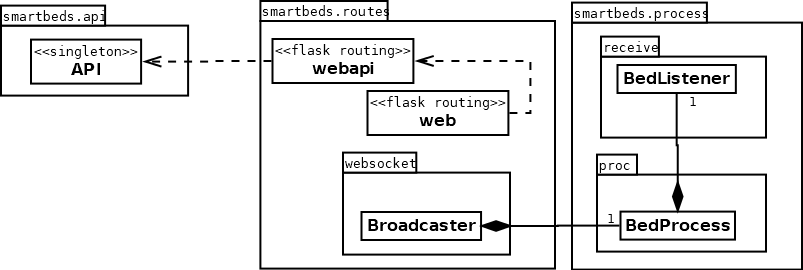
\includegraphics[width=\textwidth]{classes}
	\caption{Diagrama de clases}
	\label{fig:classes}
\end{figure}

La arquitectura global de la aplicación sigue el diagrama de componentes de la figura~\ref{fig:despl}. La aplicación, desarrollada en la librería de \textit{Python}, \textit{Flask}, se conecta a una base de datos relacional compatible con la API de \textit{MySQL}, en el caso concreto del despliegue actual se usa la implementación de \textit{MariaDB}; la aplicación también lanza hilos para la escucha de camas mediante multidifusión, aunque el diagrama solo tiene una pueden ser tantas como se requiera. El último módulo es el servidor web, en el caso del despliegue actual es un \textit{Nginx} pero puede ser cualquiera, lo que debe ser de proxy reverso.

\begin{figure}
	\centering
	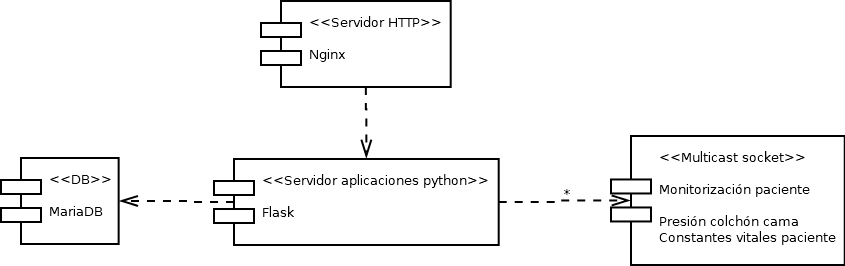
\includegraphics[width=\textwidth]{despliegue}
	\caption{Diagrama de despliegue}
	\label{fig:despl}
\end{figure}



\section{Diseño de interfaces}

Las interfaces se han diseñado teniendo en cuenta la usabilidad de la misma así como un diseño simple que permitiese que fuese más intuitiva con una curva de aprendizaje leve. Se ha tenido en cuenta también que la interfaz sea adaptable a una gran variedad de pantallas teniendo en cuenta que, al ser una aplicación web, el uso de la misma puede ser en multitud de dispositivos diferentes (diseño \textit{responsive}~\cite{wiki:responsive}).

Los primeros prototipos fueron realizados sobre el caso de uso especificado en la tabla~\ref{tabla:tablaCU22}, tanto para escritorio (imagen~\ref{fig:proto-desk}) como para móvil (imagen~\ref{fig:proto-mob}).

\begin{figure}[h]
	\centering
	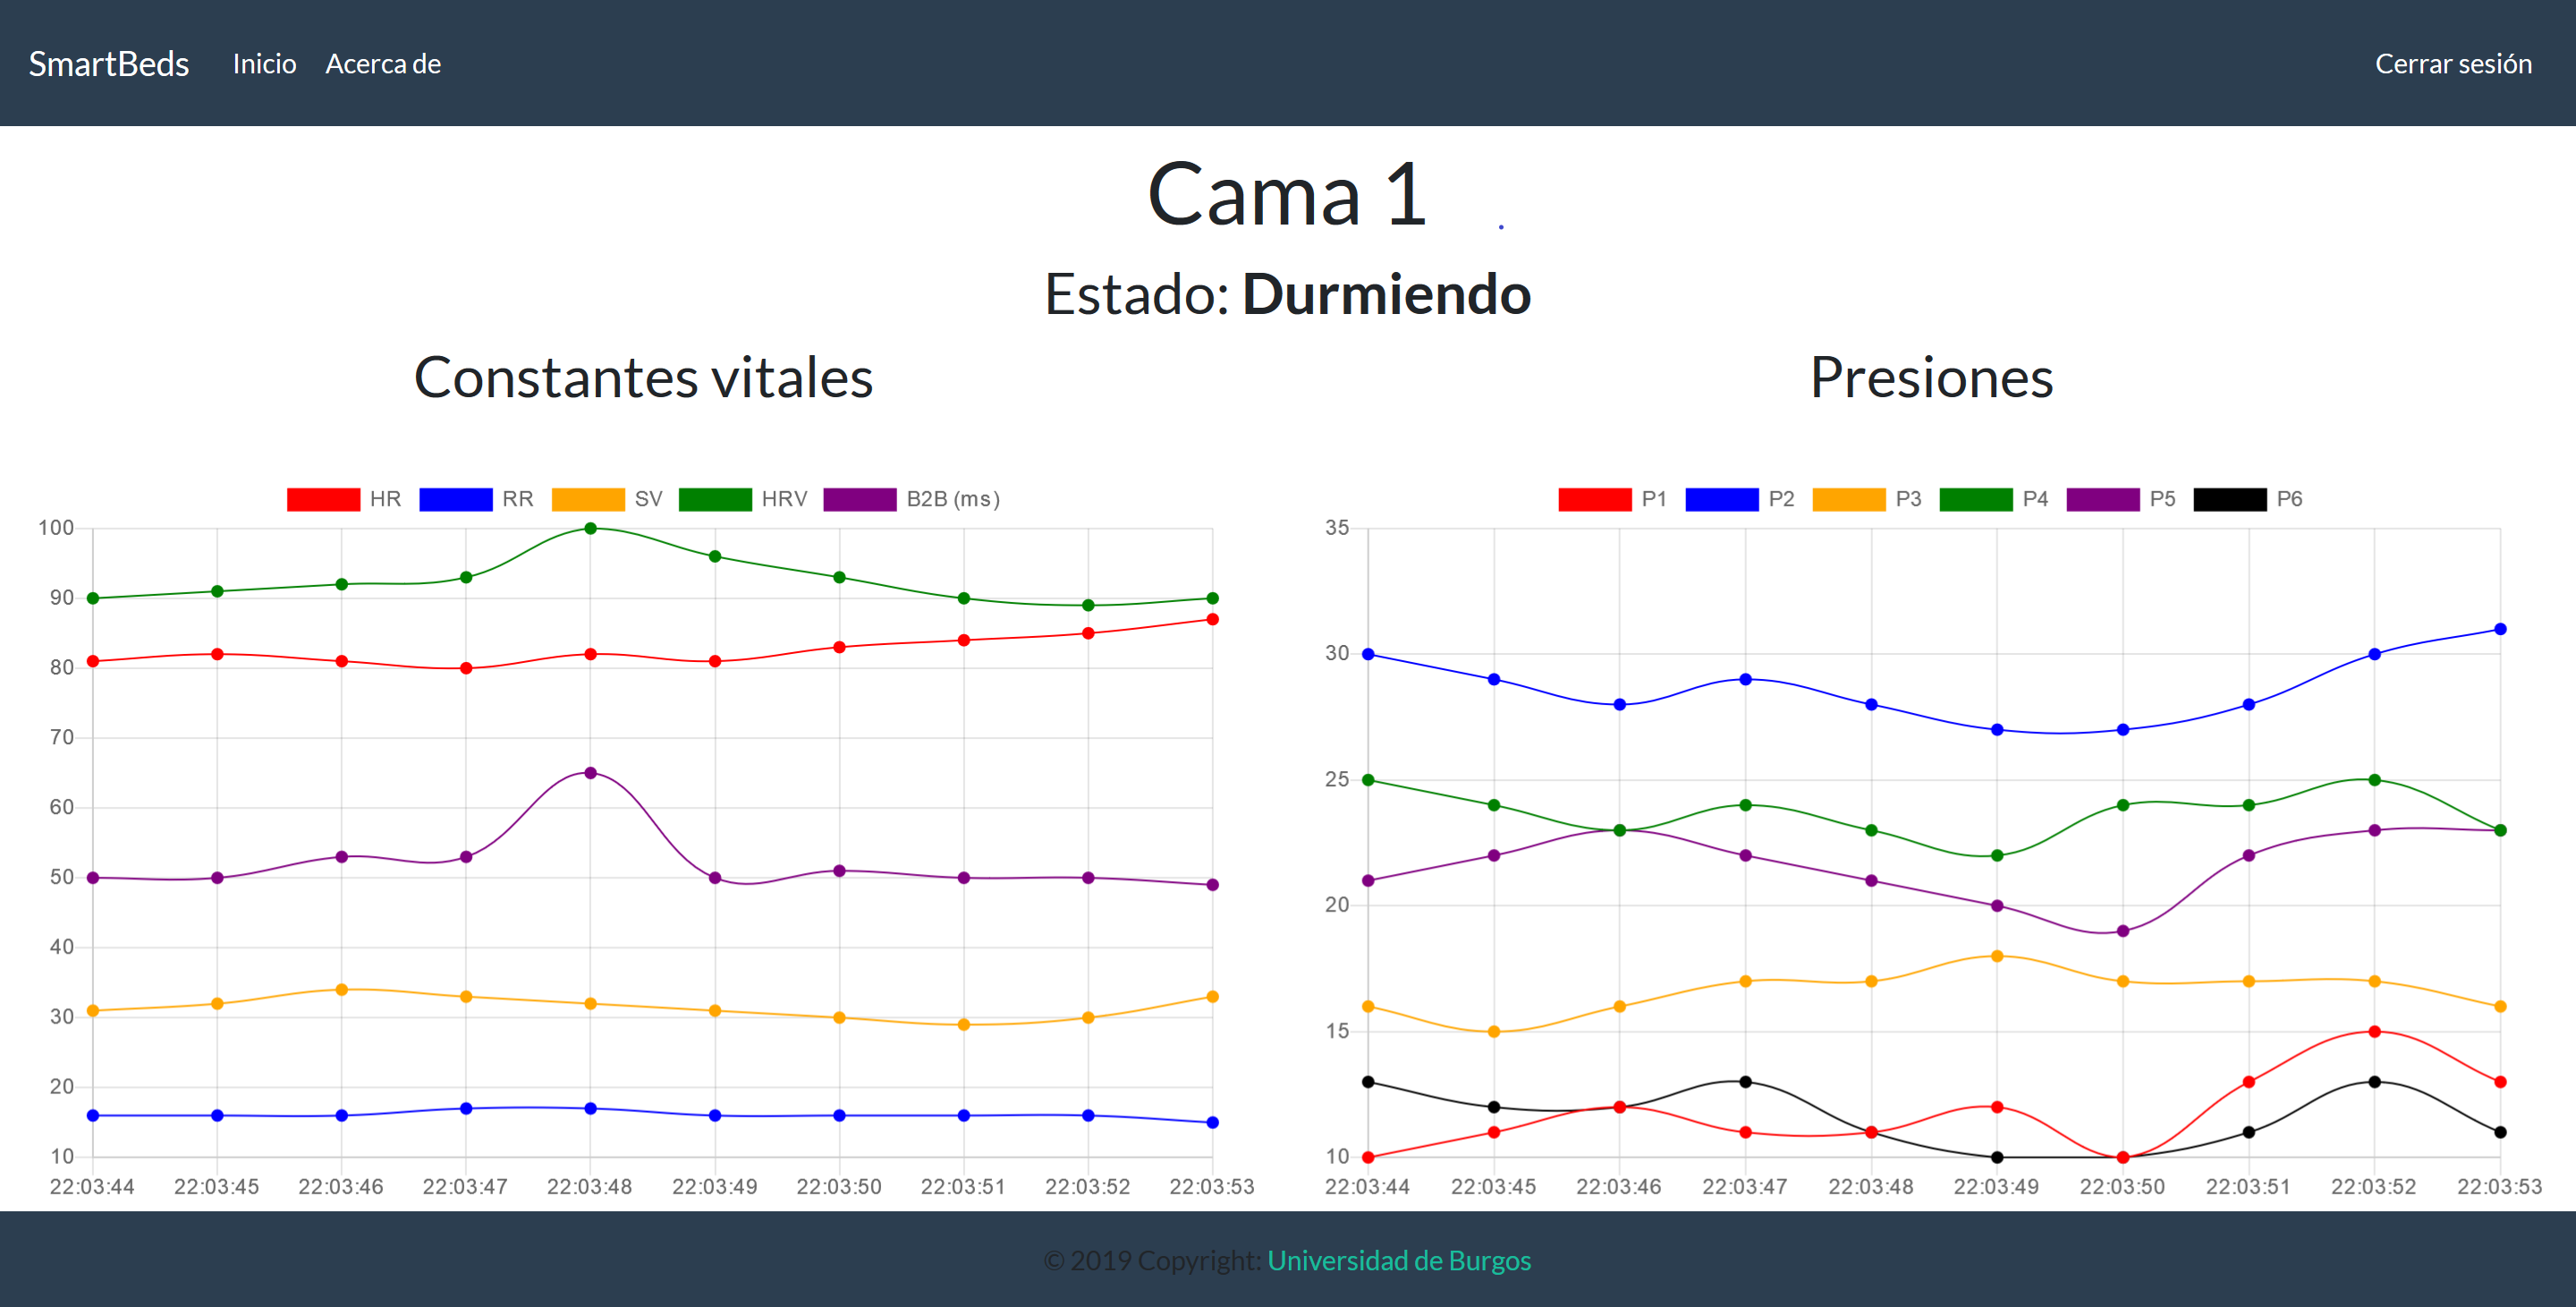
\includegraphics[width=\textwidth]{prot-desktop}
	\caption{Prototipo para escritorio}
	\label{fig:proto-desk}
\end{figure}

\begin{figure}[h]
	\centering
	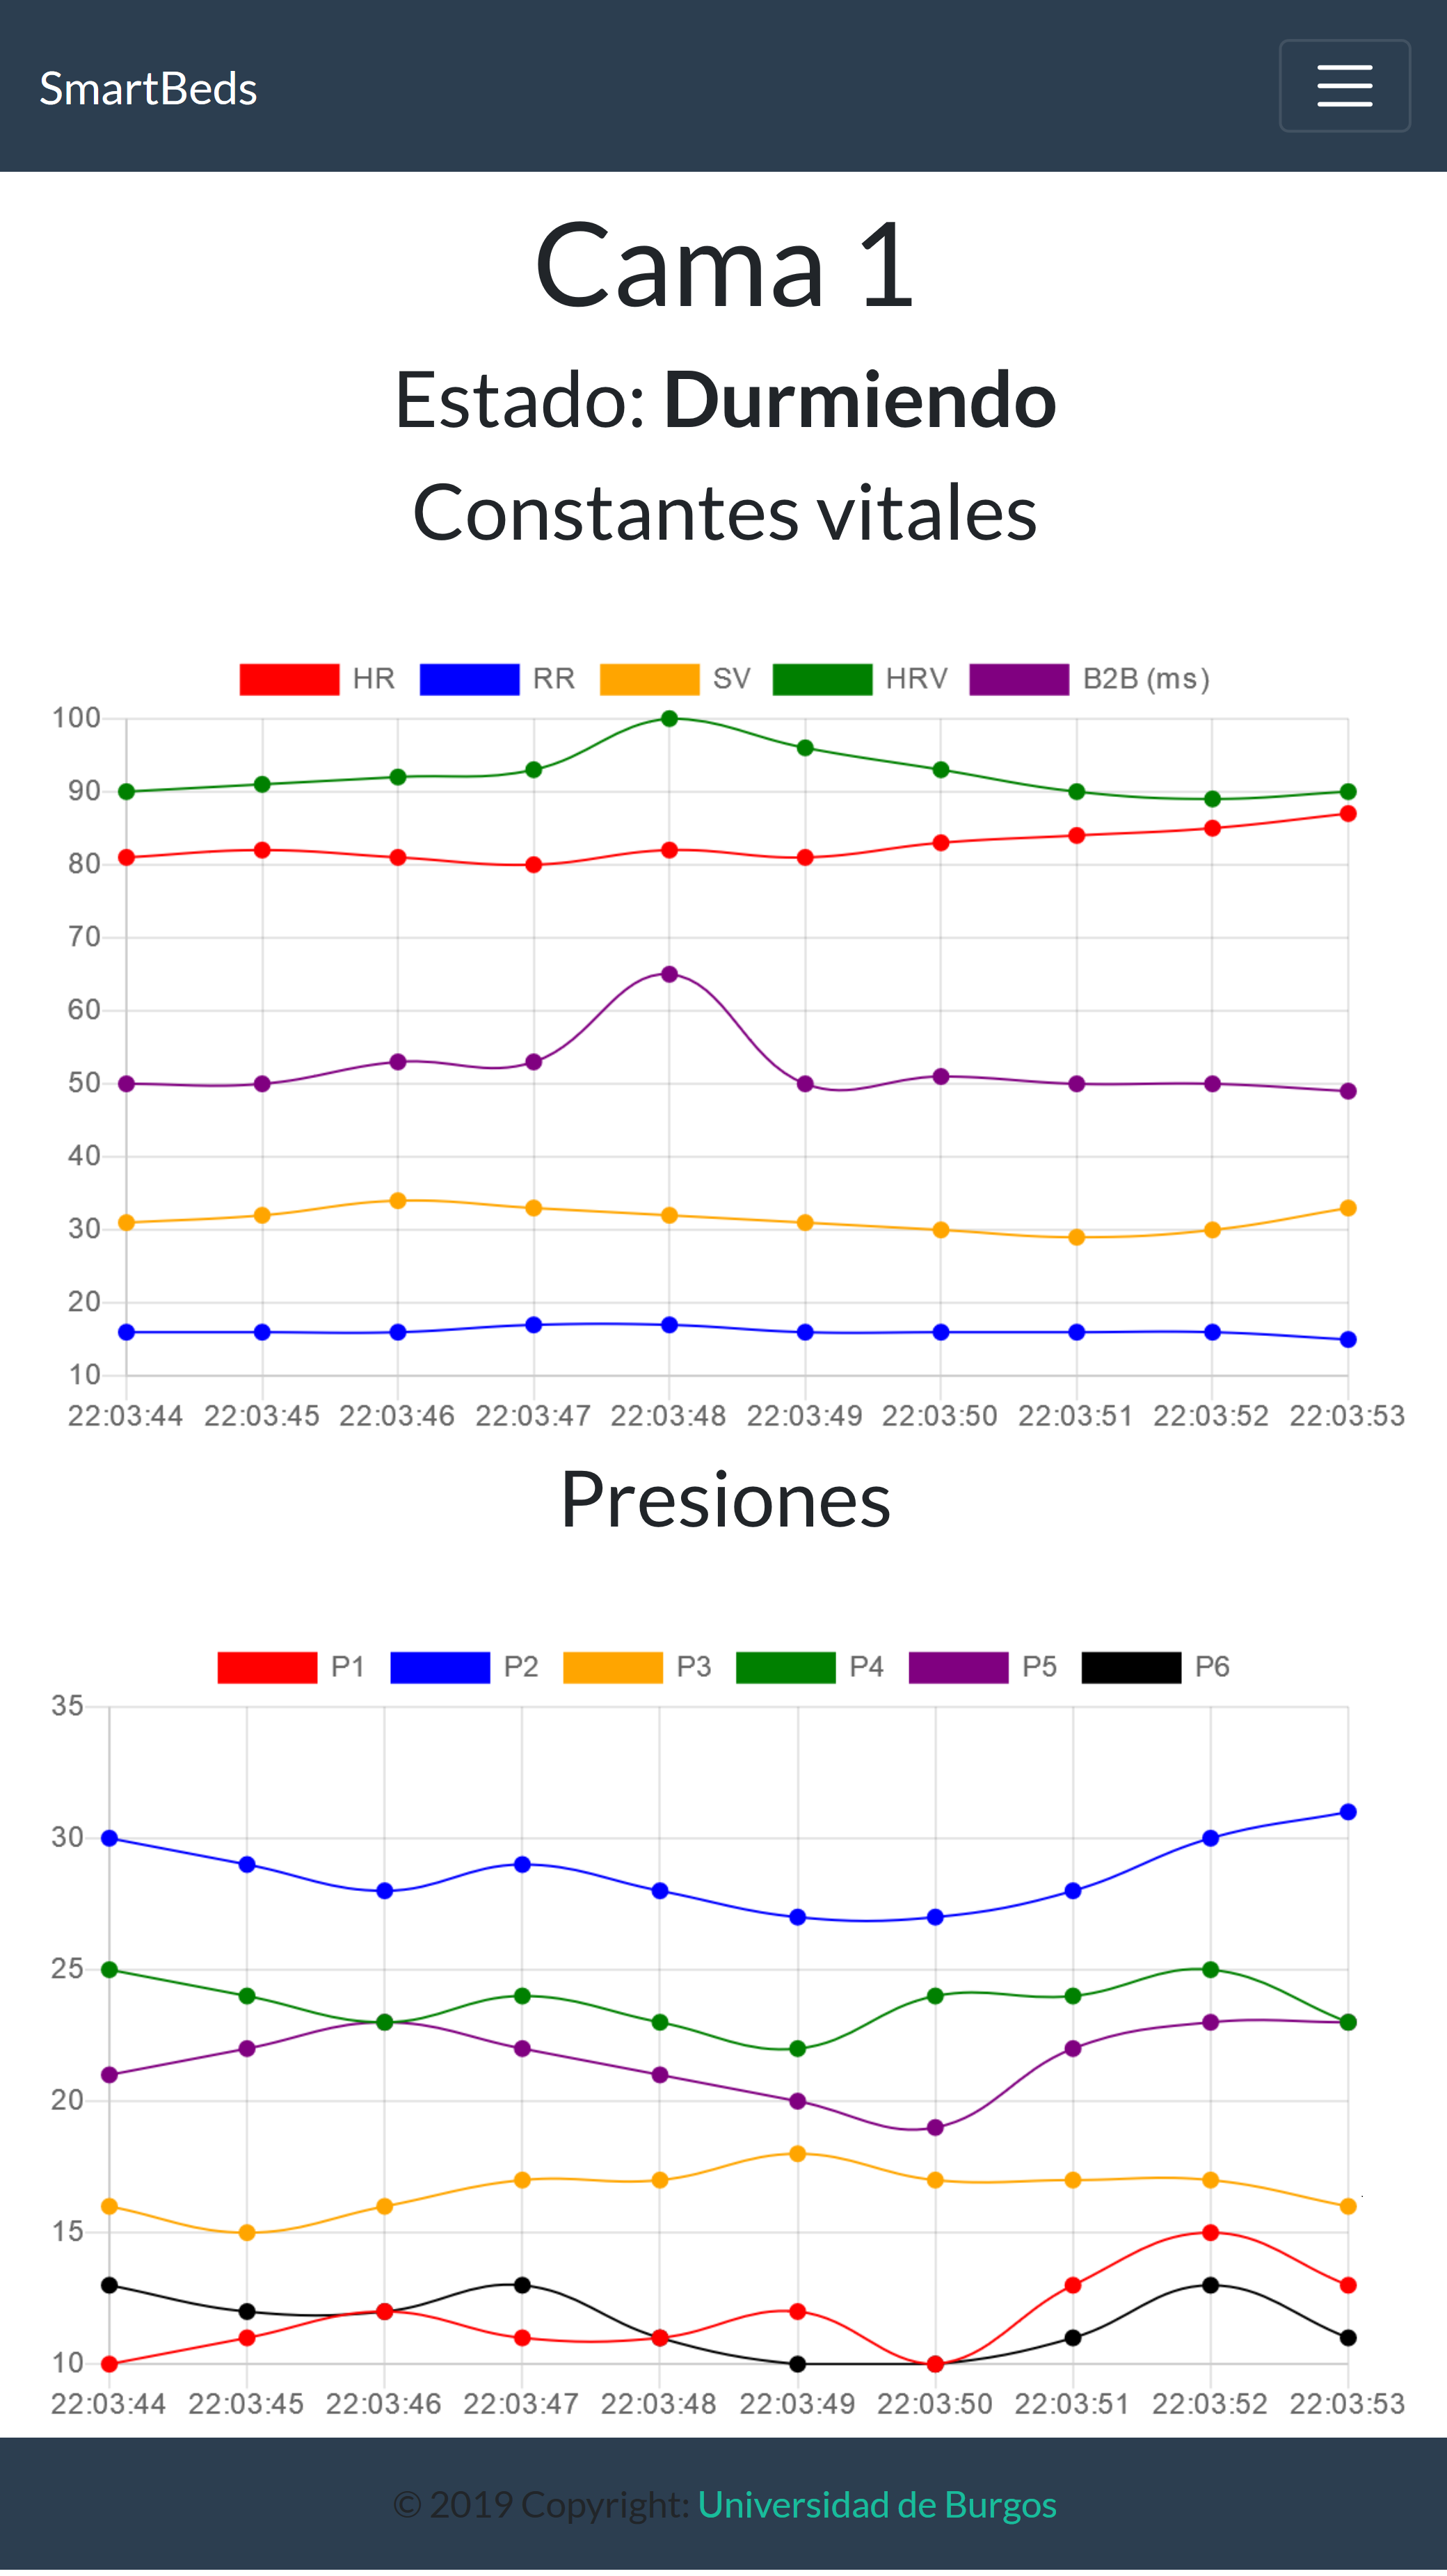
\includegraphics[width=0.45\textwidth]{prot-mobile}
	\caption{Prototipo para móvil}
	\label{fig:proto-mob}
\end{figure}
